\section{Success Case: en-fr on the Strict-Filter v1 Corpus}
\label{sec:enfr_v1}

This section reports the two success runs that establish the clean-data baseline of the 2x2: Base v1.1 and Big v1.1 on the strict-filter 9.3M en-fr corpus. Both land within or above the sacrebleu-equivalent of the original paper's reported BLEU, and Big exceeds Base by $+0.56$ test BLEU.

\subsection{Corpus construction}
\label{sec:v1_corpus}
The v1 corpus consists of the first 10M raw pairs of WMT14 en-fr (HuggingFace Datasets stream order, deterministic), passed through our default cleaning script (\S\ref{sec:setup}). 9.3M pairs survive (93\% keep rate). The 10M cap was originally an accident inherited from an earlier zh-en experiment; we retain it because the resulting 9.3M sits comfortably above the smallest-effective-corpus zone for Base Transformer training, yet remains small enough to fall clearly in the ``data-limited'' regime where data quality dominates.

A first version of v1 (call it v1.0) used \texttt{character\_coverage=0.9995} for the SPM, which mapped $\sim$~4.4\% of accented French validation tokens to \texttt{<unk>} (e.g.\ \textit{Israël} $\rightarrow$ \texttt{Isra ?? l}). This cost $\sim$~0.5 BLEU at the headline. Our v1.1 numbers fix this with \texttt{character\_coverage=1.0}; v1.0 figures are listed for provenance only --- the paper's analysis uses v1.1 throughout.

\subsection{Base v1.1: 60M parameters}
\label{sec:base_v1}
Trained from scratch for 100K steps under the schedule of \S\ref{sec:setup}; best converged valid BLEU was 29.83 (single ckpt). Extending the schedule to 122K steps under the same Noam decay lifted the curve modestly (best 30.21). Averaging the last 5 checkpoints adds 0.69 BLEU on valid (averaged: 30.52); test newstest2014 is 35.31. Total wall-clock: 2~h~30~min on the 5090.

The training curve (Figure~\ref{fig:base_v1_curves}) shows the canonical Vaswani shape: a Noam ramp to peak $\approx 7\text{e-}4$ at step 4K, then $1/\sqrt{\text{step}}$ decay through 122K. Loss falls smoothly to $\sim$~3.3, with no spike-guard triggers in 122K steps (\S\ref{sec:methodology}).

\begin{figure}[t]
\centering
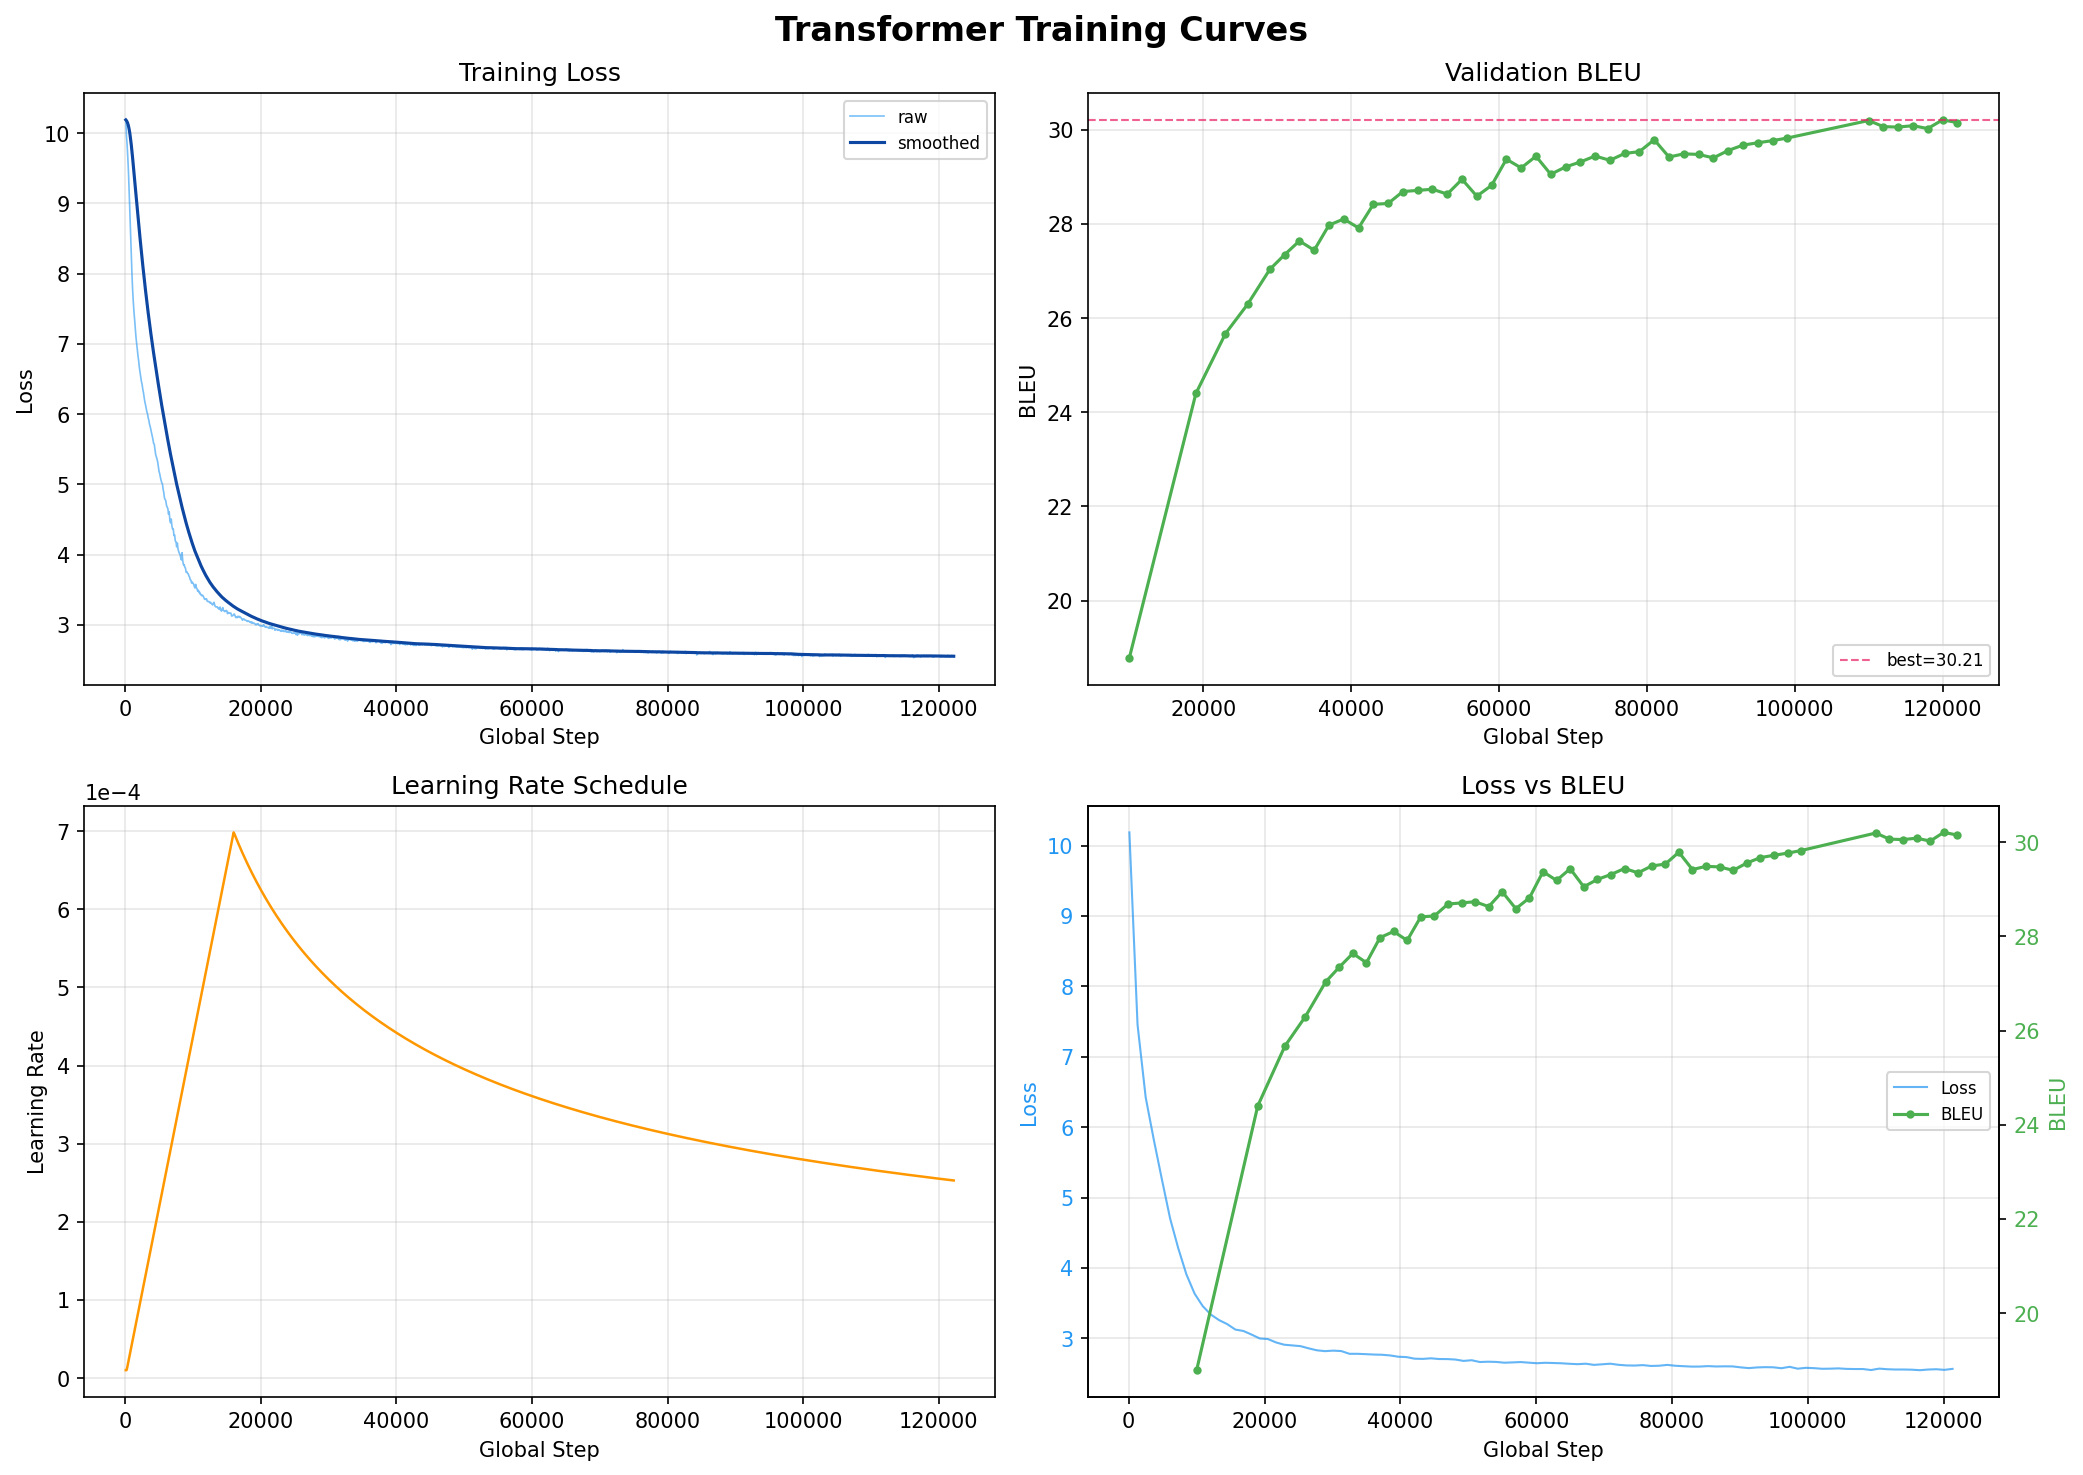
\includegraphics[width=\columnwidth]{figures/base_v1_curves.png}
\caption{Base v1.1 training curves (60M parameters, 122K steps, 9.3M strict-filter en-fr corpus). Top-left: training loss; top-right: validation BLEU (newstest2013) climbing monotonically through 30.21; bottom-left: Noam learning-rate schedule with peak $\approx 7\text{e-}4$ at warmup step 4K; bottom-right: loss/BLEU joint view. Zero spike-guard activations across the run.}
\label{fig:base_v1_curves}
\end{figure}

\subsection{Big v1.1: 209M parameters, same data}
\label{sec:big_v1}
Trained from scratch for 280K steps with the same data, SPM, and eval pipeline; early-stopped at 260K under patience. Best single-checkpoint valid is 30.69. Averaging 5 checkpoints in [210K, 250K] gives valid 31.14 / test 35.87. Total wall-clock: 6~h on the 5090.

\begin{figure}[t]
\centering
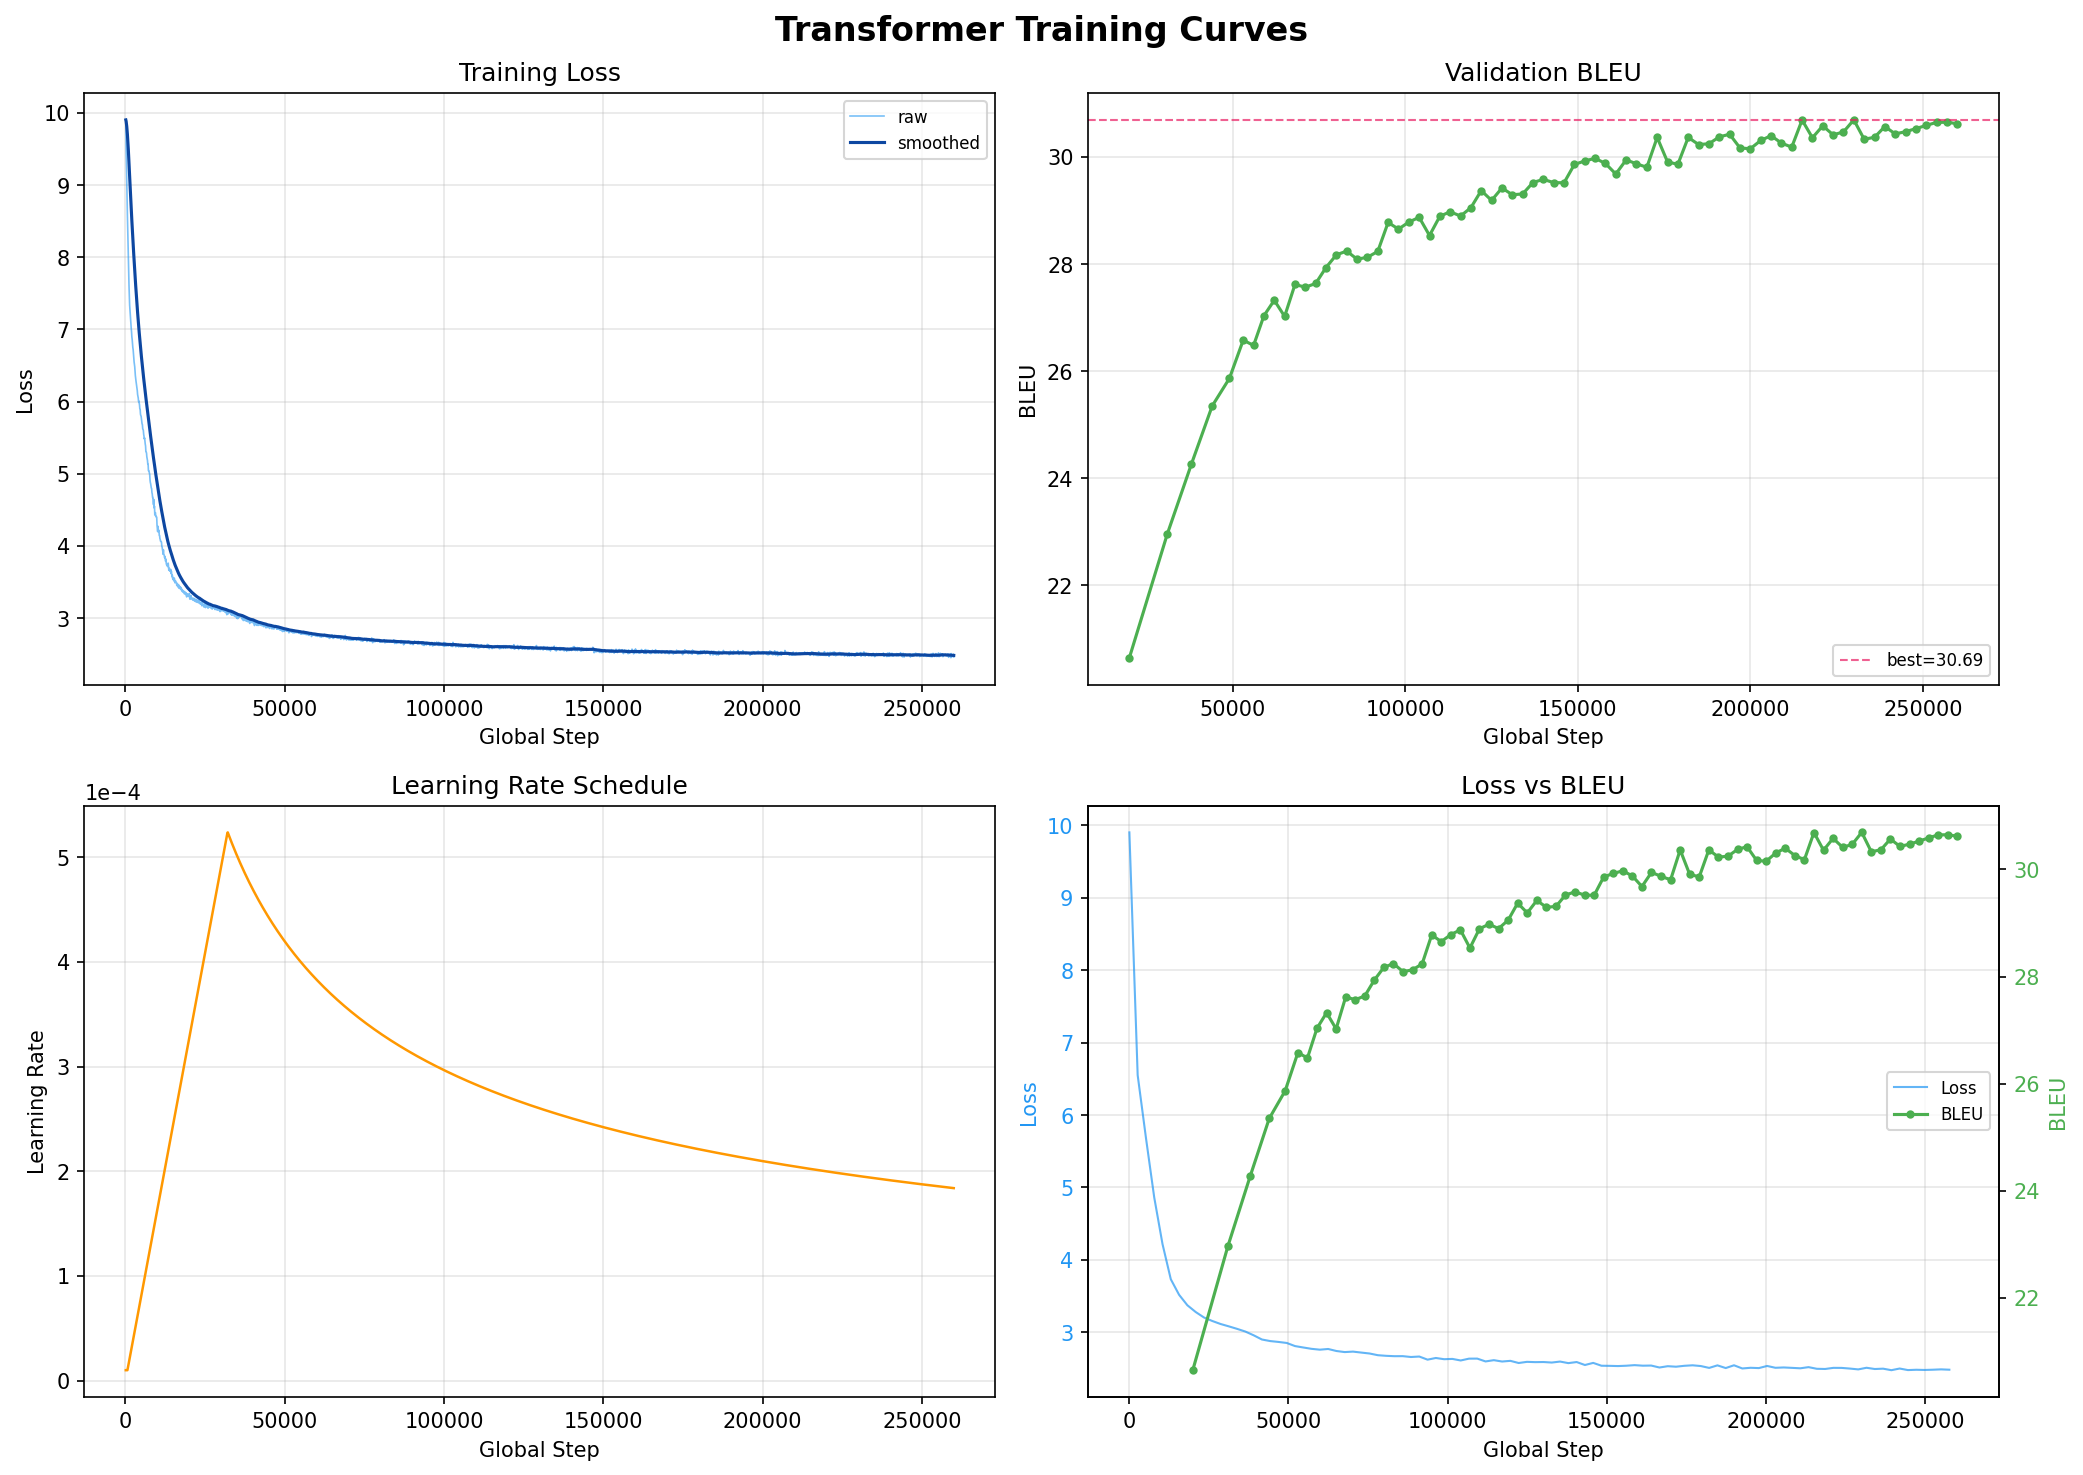
\includegraphics[width=\columnwidth]{figures/big_v1_curves.png}
\caption{Big v1.1 training curves (209M parameters, early-stopped at 260K of 280K planned, same 9.3M strict-filter en-fr corpus as Base v1.1). Validation BLEU plateaus around 30.5--30.7 from step 200K onwards; training-loss floor reaches $\sim$~2.3 (vs.\ Base v1.1's $\sim$~3.3). The lower loss floor at greater capacity is the data point exploited in \S\ref{sec:methodology}.}
\label{fig:big_v1_curves}
\end{figure}

\subsection{Capacity gap on clean data}
\label{sec:v1_capacity}

\begin{table}[t]
\centering
\small
\begin{tabular}{lrrr}
\toprule
\textbf{Run} & \textbf{Params} & \textbf{Valid} & \textbf{Test} \\
\midrule
Base v1.1 & 60M  & 30.52 & 35.31 \\
Big  v1.1 & 209M & 31.14 & 35.87 \\
\midrule
$\Delta$ (Big $-$ Base) & $+3.5\times$ & $+0.62$ & $\mathbf{+0.56}$ \\
\bottomrule
\end{tabular}
\caption{Capacity gap on the clean v1.1 corpus. BLEU on newstest2013 (valid) / newstest2014 (test); sacrebleu 13a, beam=5, length-penalty=1.0, 5-checkpoint averaged. Big exceeds Base by $+0.56$ BLEU on test.}
\label{tab:v1_capacity}
\end{table}

The $+0.56$ test gap is the ``capacity pays'' baseline of the 2x2. \S\ref{sec:enfr_v2} will show that on the loose-filter v2 corpus the same architectural change costs $-0.87$ BLEU, flipping the sign.

The gap is small in absolute terms compared to typical contemporary scaling reports, but it is consistent with the original paper's $\sim$~1 tokenized-BLEU Big-over-Base gap on en-fr (Vaswani 38.1 Big vs 37.0 Base $\approx$ +1.1 tokenized $\approx$ +0.5--0.7 sacrebleu). The relative scaling magnitude is preserved; the next section shows that this magnitude depends on the data being clean.

\subsection{Provenance: v1.0 numbers (retired)}
For reference: v1.0 (with \texttt{character\_coverage=0.9995}, 100K steps) reached test 34.69 (Base) / 34.66 (Big) --- the two sat within noise on the same data, which we initially interpreted as a ``shared tokenizer ceiling''. The v1.1 numbers (35.31 / 35.87) show that this was a tokenizer artifact rather than a capacity ceiling: with the tokenizer fixed, Big cleanly separates from Base. We retain v1.0 only as historical context; all subsequent analysis uses v1.1.
